% Graphic for TeX using PGF
% Title: /home/budnyjj/univer/GIT/diploma/b/design/diagrams/ui_edit_manager.dia
% Creator: Dia v0.97.3
% CreationDate: Sun May  8 02:21:02 2016
% For: budnyjj
% \usepackage{tikz}
% The following commands are not supported in PSTricks at present
% We define them conditionally, so when they are implemented,
% this pgf file will use them.
\ifx\du\undefined
  \newlength{\du}
\fi
\setlength{\du}{15\unitlength}
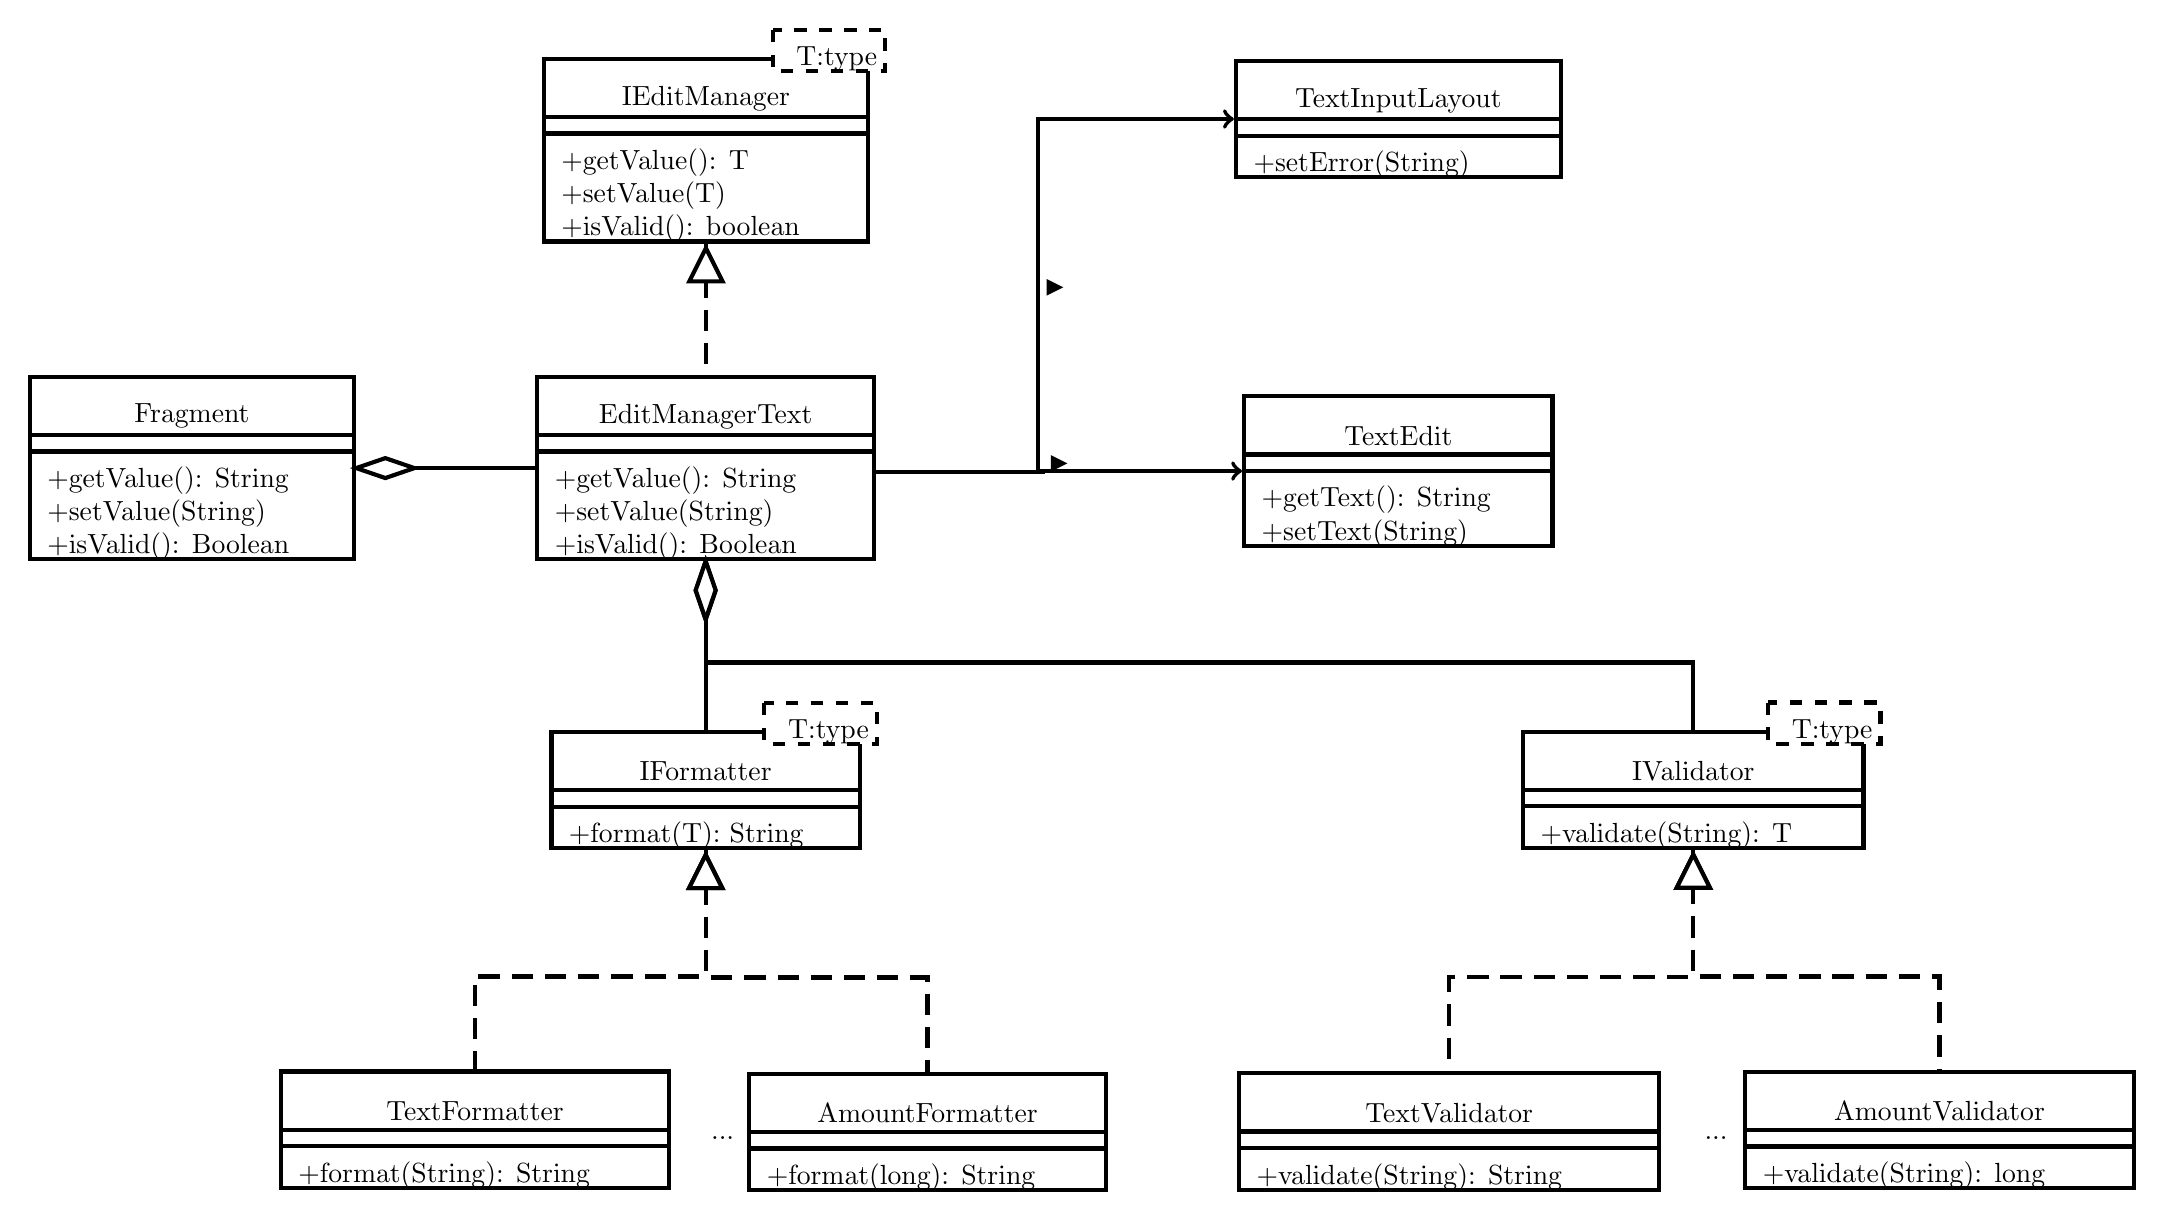
\begin{tikzpicture}
\pgftransformxscale{1.000000}
\pgftransformyscale{-1.000000}
\definecolor{dialinecolor}{rgb}{0.000000, 0.000000, 0.000000}
\pgfsetstrokecolor{dialinecolor}
\definecolor{dialinecolor}{rgb}{1.000000, 1.000000, 1.000000}
\pgfsetfillcolor{dialinecolor}
\pgfsetlinewidth{0.100000\du}
\pgfsetdash{}{0pt}
\definecolor{dialinecolor}{rgb}{1.000000, 1.000000, 1.000000}
\pgfsetfillcolor{dialinecolor}
\fill (17.408060\du,36.291988\du)--(17.408060\du,37.691988\du)--(24.838060\du,37.691988\du)--(24.838060\du,36.291988\du)--cycle;
\definecolor{dialinecolor}{rgb}{0.000000, 0.000000, 0.000000}
\pgfsetstrokecolor{dialinecolor}
\draw (17.408060\du,36.291988\du)--(17.408060\du,37.691988\du)--(24.838060\du,37.691988\du)--(24.838060\du,36.291988\du)--cycle;
% setfont left to latex
\definecolor{dialinecolor}{rgb}{0.000000, 0.000000, 0.000000}
\pgfsetstrokecolor{dialinecolor}
\node at (21.123060\du,37.241988\du){IFormatter};
\definecolor{dialinecolor}{rgb}{1.000000, 1.000000, 1.000000}
\pgfsetfillcolor{dialinecolor}
\fill (17.408060\du,37.691988\du)--(17.408060\du,38.091988\du)--(24.838060\du,38.091988\du)--(24.838060\du,37.691988\du)--cycle;
\definecolor{dialinecolor}{rgb}{0.000000, 0.000000, 0.000000}
\pgfsetstrokecolor{dialinecolor}
\draw (17.408060\du,37.691988\du)--(17.408060\du,38.091988\du)--(24.838060\du,38.091988\du)--(24.838060\du,37.691988\du)--cycle;
\definecolor{dialinecolor}{rgb}{1.000000, 1.000000, 1.000000}
\pgfsetfillcolor{dialinecolor}
\fill (17.408060\du,38.091988\du)--(17.408060\du,39.091988\du)--(24.838060\du,39.091988\du)--(24.838060\du,38.091988\du)--cycle;
\definecolor{dialinecolor}{rgb}{0.000000, 0.000000, 0.000000}
\pgfsetstrokecolor{dialinecolor}
\draw (17.408060\du,38.091988\du)--(17.408060\du,39.091988\du)--(24.838060\du,39.091988\du)--(24.838060\du,38.091988\du)--cycle;
% setfont left to latex
\definecolor{dialinecolor}{rgb}{0.000000, 0.000000, 0.000000}
\pgfsetstrokecolor{dialinecolor}
\node[anchor=west] at (17.558060\du,38.791988\du){+format(T): String};
\definecolor{dialinecolor}{rgb}{1.000000, 1.000000, 1.000000}
\pgfsetfillcolor{dialinecolor}
\fill (22.538060\du,35.591988\du)--(22.538060\du,36.591988\du)--(25.248060\du,36.591988\du)--(25.248060\du,35.591988\du)--cycle;
\pgfsetdash{{1.000000\du}{1.000000\du}}{0\du}
\pgfsetdash{{0.300000\du}{0.300000\du}}{0\du}
\definecolor{dialinecolor}{rgb}{0.000000, 0.000000, 0.000000}
\pgfsetstrokecolor{dialinecolor}
\draw (22.538060\du,35.591988\du)--(22.538060\du,36.591988\du)--(25.248060\du,36.591988\du)--(25.248060\du,35.591988\du)--cycle;
% setfont left to latex
\definecolor{dialinecolor}{rgb}{0.000000, 0.000000, 0.000000}
\pgfsetstrokecolor{dialinecolor}
\node[anchor=west] at (22.838060\du,36.291988\du){T:type};
\pgfsetlinewidth{0.100000\du}
\pgfsetdash{}{0pt}
\definecolor{dialinecolor}{rgb}{1.000000, 1.000000, 1.000000}
\pgfsetfillcolor{dialinecolor}
\fill (10.889288\du,44.471452\du)--(10.889288\du,45.871452\du)--(20.244288\du,45.871452\du)--(20.244288\du,44.471452\du)--cycle;
\definecolor{dialinecolor}{rgb}{0.000000, 0.000000, 0.000000}
\pgfsetstrokecolor{dialinecolor}
\draw (10.889288\du,44.471452\du)--(10.889288\du,45.871452\du)--(20.244288\du,45.871452\du)--(20.244288\du,44.471452\du)--cycle;
% setfont left to latex
\definecolor{dialinecolor}{rgb}{0.000000, 0.000000, 0.000000}
\pgfsetstrokecolor{dialinecolor}
\node at (15.566788\du,45.421452\du){TextFormatter};
\definecolor{dialinecolor}{rgb}{1.000000, 1.000000, 1.000000}
\pgfsetfillcolor{dialinecolor}
\fill (10.889288\du,45.871452\du)--(10.889288\du,46.271452\du)--(20.244288\du,46.271452\du)--(20.244288\du,45.871452\du)--cycle;
\definecolor{dialinecolor}{rgb}{0.000000, 0.000000, 0.000000}
\pgfsetstrokecolor{dialinecolor}
\draw (10.889288\du,45.871452\du)--(10.889288\du,46.271452\du)--(20.244288\du,46.271452\du)--(20.244288\du,45.871452\du)--cycle;
\definecolor{dialinecolor}{rgb}{1.000000, 1.000000, 1.000000}
\pgfsetfillcolor{dialinecolor}
\fill (10.889288\du,46.271452\du)--(10.889288\du,47.271452\du)--(20.244288\du,47.271452\du)--(20.244288\du,46.271452\du)--cycle;
\definecolor{dialinecolor}{rgb}{0.000000, 0.000000, 0.000000}
\pgfsetstrokecolor{dialinecolor}
\draw (10.889288\du,46.271452\du)--(10.889288\du,47.271452\du)--(20.244288\du,47.271452\du)--(20.244288\du,46.271452\du)--cycle;
% setfont left to latex
\definecolor{dialinecolor}{rgb}{0.000000, 0.000000, 0.000000}
\pgfsetstrokecolor{dialinecolor}
\node[anchor=west] at (11.039288\du,46.971452\du){+format(String): String};
\pgfsetlinewidth{0.100000\du}
\pgfsetdash{}{0pt}
\definecolor{dialinecolor}{rgb}{1.000000, 1.000000, 1.000000}
\pgfsetfillcolor{dialinecolor}
\fill (22.174163\du,44.526037\du)--(22.174163\du,45.926037\du)--(30.759163\du,45.926037\du)--(30.759163\du,44.526037\du)--cycle;
\definecolor{dialinecolor}{rgb}{0.000000, 0.000000, 0.000000}
\pgfsetstrokecolor{dialinecolor}
\draw (22.174163\du,44.526037\du)--(22.174163\du,45.926037\du)--(30.759163\du,45.926037\du)--(30.759163\du,44.526037\du)--cycle;
% setfont left to latex
\definecolor{dialinecolor}{rgb}{0.000000, 0.000000, 0.000000}
\pgfsetstrokecolor{dialinecolor}
\node at (26.466663\du,45.476037\du){AmountFormatter};
\definecolor{dialinecolor}{rgb}{1.000000, 1.000000, 1.000000}
\pgfsetfillcolor{dialinecolor}
\fill (22.174163\du,45.926037\du)--(22.174163\du,46.326037\du)--(30.759163\du,46.326037\du)--(30.759163\du,45.926037\du)--cycle;
\definecolor{dialinecolor}{rgb}{0.000000, 0.000000, 0.000000}
\pgfsetstrokecolor{dialinecolor}
\draw (22.174163\du,45.926037\du)--(22.174163\du,46.326037\du)--(30.759163\du,46.326037\du)--(30.759163\du,45.926037\du)--cycle;
\definecolor{dialinecolor}{rgb}{1.000000, 1.000000, 1.000000}
\pgfsetfillcolor{dialinecolor}
\fill (22.174163\du,46.326037\du)--(22.174163\du,47.326037\du)--(30.759163\du,47.326037\du)--(30.759163\du,46.326037\du)--cycle;
\definecolor{dialinecolor}{rgb}{0.000000, 0.000000, 0.000000}
\pgfsetstrokecolor{dialinecolor}
\draw (22.174163\du,46.326037\du)--(22.174163\du,47.326037\du)--(30.759163\du,47.326037\du)--(30.759163\du,46.326037\du)--cycle;
% setfont left to latex
\definecolor{dialinecolor}{rgb}{0.000000, 0.000000, 0.000000}
\pgfsetstrokecolor{dialinecolor}
\node[anchor=west] at (22.324163\du,47.026037\du){+format(long): String};
\pgfsetlinewidth{0.100000\du}
\pgfsetdash{{0.300000\du}{0.300000\du}}{0\du}
\pgfsetdash{{0.400000\du}{0.400000\du}}{0\du}
\pgfsetmiterjoin
\pgfsetbuttcap
{
\definecolor{dialinecolor}{rgb}{0.000000, 0.000000, 0.000000}
\pgfsetfillcolor{dialinecolor}
% was here!!!
\definecolor{dialinecolor}{rgb}{0.000000, 0.000000, 0.000000}
\pgfsetstrokecolor{dialinecolor}
\draw (21.123060\du,39.142342\du)--(21.123060\du,42.181720\du)--(15.566788\du,42.181720\du)--(15.566788\du,44.421098\du);
}
\definecolor{dialinecolor}{rgb}{0.000000, 0.000000, 0.000000}
\pgfsetstrokecolor{dialinecolor}
\draw (21.123060\du,40.054146\du)--(21.123060\du,42.181720\du)--(15.566788\du,42.181720\du)--(15.566788\du,44.421098\du);
\pgfsetmiterjoin
\definecolor{dialinecolor}{rgb}{1.000000, 1.000000, 1.000000}
\pgfsetfillcolor{dialinecolor}
\fill (21.523060\du,40.054146\du)--(21.123060\du,39.254146\du)--(20.723060\du,40.054146\du)--cycle;
\pgfsetlinewidth{0.100000\du}
\pgfsetdash{}{0pt}
\pgfsetmiterjoin
\definecolor{dialinecolor}{rgb}{0.000000, 0.000000, 0.000000}
\pgfsetstrokecolor{dialinecolor}
\draw (21.523060\du,40.054146\du)--(21.123060\du,39.254146\du)--(20.723060\du,40.054146\du)--cycle;
% setfont left to latex
\pgfsetlinewidth{0.100000\du}
\pgfsetdash{{0.400000\du}{0.400000\du}}{0\du}
\pgfsetdash{{0.400000\du}{0.400000\du}}{0\du}
\pgfsetmiterjoin
\pgfsetbuttcap
{
\definecolor{dialinecolor}{rgb}{0.000000, 0.000000, 0.000000}
\pgfsetfillcolor{dialinecolor}
% was here!!!
\definecolor{dialinecolor}{rgb}{0.000000, 0.000000, 0.000000}
\pgfsetstrokecolor{dialinecolor}
\draw (21.123060\du,39.142342\du)--(21.123060\du,42.209013\du)--(26.466663\du,42.209013\du)--(26.466663\du,44.475683\du);
}
\definecolor{dialinecolor}{rgb}{0.000000, 0.000000, 0.000000}
\pgfsetstrokecolor{dialinecolor}
\draw (21.123060\du,40.054146\du)--(21.123060\du,42.209013\du)--(26.466663\du,42.209013\du)--(26.466663\du,44.475683\du);
\pgfsetmiterjoin
\definecolor{dialinecolor}{rgb}{1.000000, 1.000000, 1.000000}
\pgfsetfillcolor{dialinecolor}
\fill (21.523060\du,40.054146\du)--(21.123060\du,39.254146\du)--(20.723060\du,40.054146\du)--cycle;
\pgfsetlinewidth{0.100000\du}
\pgfsetdash{}{0pt}
\pgfsetmiterjoin
\definecolor{dialinecolor}{rgb}{0.000000, 0.000000, 0.000000}
\pgfsetstrokecolor{dialinecolor}
\draw (21.523060\du,40.054146\du)--(21.123060\du,39.254146\du)--(20.723060\du,40.054146\du)--cycle;
% setfont left to latex
\pgfsetlinewidth{0.100000\du}
\pgfsetdash{}{0pt}
\definecolor{dialinecolor}{rgb}{1.000000, 1.000000, 1.000000}
\pgfsetfillcolor{dialinecolor}
\fill (33.974181\du,44.517302\du)--(33.974181\du,45.917302\du)--(44.099181\du,45.917302\du)--(44.099181\du,44.517302\du)--cycle;
\definecolor{dialinecolor}{rgb}{0.000000, 0.000000, 0.000000}
\pgfsetstrokecolor{dialinecolor}
\draw (33.974181\du,44.517302\du)--(33.974181\du,45.917302\du)--(44.099181\du,45.917302\du)--(44.099181\du,44.517302\du)--cycle;
% setfont left to latex
\definecolor{dialinecolor}{rgb}{0.000000, 0.000000, 0.000000}
\pgfsetstrokecolor{dialinecolor}
\node at (39.036681\du,45.467302\du){TextValidator};
\definecolor{dialinecolor}{rgb}{1.000000, 1.000000, 1.000000}
\pgfsetfillcolor{dialinecolor}
\fill (33.974181\du,45.917302\du)--(33.974181\du,46.317302\du)--(44.099181\du,46.317302\du)--(44.099181\du,45.917302\du)--cycle;
\definecolor{dialinecolor}{rgb}{0.000000, 0.000000, 0.000000}
\pgfsetstrokecolor{dialinecolor}
\draw (33.974181\du,45.917302\du)--(33.974181\du,46.317302\du)--(44.099181\du,46.317302\du)--(44.099181\du,45.917302\du)--cycle;
\definecolor{dialinecolor}{rgb}{1.000000, 1.000000, 1.000000}
\pgfsetfillcolor{dialinecolor}
\fill (33.974181\du,46.317302\du)--(33.974181\du,47.317302\du)--(44.099181\du,47.317302\du)--(44.099181\du,46.317302\du)--cycle;
\definecolor{dialinecolor}{rgb}{0.000000, 0.000000, 0.000000}
\pgfsetstrokecolor{dialinecolor}
\draw (33.974181\du,46.317302\du)--(33.974181\du,47.317302\du)--(44.099181\du,47.317302\du)--(44.099181\du,46.317302\du)--cycle;
% setfont left to latex
\definecolor{dialinecolor}{rgb}{0.000000, 0.000000, 0.000000}
\pgfsetstrokecolor{dialinecolor}
\node[anchor=west] at (34.124181\du,47.017302\du){+validate(String): String};
\pgfsetlinewidth{0.100000\du}
\pgfsetdash{}{0pt}
\definecolor{dialinecolor}{rgb}{1.000000, 1.000000, 1.000000}
\pgfsetfillcolor{dialinecolor}
\fill (46.169858\du,44.480187\du)--(46.169858\du,45.880187\du)--(55.524858\du,45.880187\du)--(55.524858\du,44.480187\du)--cycle;
\definecolor{dialinecolor}{rgb}{0.000000, 0.000000, 0.000000}
\pgfsetstrokecolor{dialinecolor}
\draw (46.169858\du,44.480187\du)--(46.169858\du,45.880187\du)--(55.524858\du,45.880187\du)--(55.524858\du,44.480187\du)--cycle;
% setfont left to latex
\definecolor{dialinecolor}{rgb}{0.000000, 0.000000, 0.000000}
\pgfsetstrokecolor{dialinecolor}
\node at (50.847358\du,45.430187\du){AmountValidator};
\definecolor{dialinecolor}{rgb}{1.000000, 1.000000, 1.000000}
\pgfsetfillcolor{dialinecolor}
\fill (46.169858\du,45.880187\du)--(46.169858\du,46.280187\du)--(55.524858\du,46.280187\du)--(55.524858\du,45.880187\du)--cycle;
\definecolor{dialinecolor}{rgb}{0.000000, 0.000000, 0.000000}
\pgfsetstrokecolor{dialinecolor}
\draw (46.169858\du,45.880187\du)--(46.169858\du,46.280187\du)--(55.524858\du,46.280187\du)--(55.524858\du,45.880187\du)--cycle;
\definecolor{dialinecolor}{rgb}{1.000000, 1.000000, 1.000000}
\pgfsetfillcolor{dialinecolor}
\fill (46.169858\du,46.280187\du)--(46.169858\du,47.280187\du)--(55.524858\du,47.280187\du)--(55.524858\du,46.280187\du)--cycle;
\definecolor{dialinecolor}{rgb}{0.000000, 0.000000, 0.000000}
\pgfsetstrokecolor{dialinecolor}
\draw (46.169858\du,46.280187\du)--(46.169858\du,47.280187\du)--(55.524858\du,47.280187\du)--(55.524858\du,46.280187\du)--cycle;
% setfont left to latex
\definecolor{dialinecolor}{rgb}{0.000000, 0.000000, 0.000000}
\pgfsetstrokecolor{dialinecolor}
\node[anchor=west] at (46.319858\du,46.980187\du){+validate(String): long};
\pgfsetlinewidth{0.100000\du}
\pgfsetdash{{0.400000\du}{0.400000\du}}{0\du}
\pgfsetdash{{0.400000\du}{0.400000\du}}{0\du}
\pgfsetmiterjoin
\pgfsetbuttcap
{
\definecolor{dialinecolor}{rgb}{0.000000, 0.000000, 0.000000}
\pgfsetfillcolor{dialinecolor}
% was here!!!
\definecolor{dialinecolor}{rgb}{0.000000, 0.000000, 0.000000}
\pgfsetstrokecolor{dialinecolor}
\draw (44.916149\du,39.134912\du)--(44.916149\du,42.200930\du)--(39.036681\du,42.200930\du)--(39.036681\du,44.466948\du);
}
\definecolor{dialinecolor}{rgb}{0.000000, 0.000000, 0.000000}
\pgfsetstrokecolor{dialinecolor}
\draw (44.916149\du,40.046715\du)--(44.916149\du,42.200930\du)--(39.036681\du,42.200930\du)--(39.036681\du,44.466948\du);
\pgfsetmiterjoin
\definecolor{dialinecolor}{rgb}{1.000000, 1.000000, 1.000000}
\pgfsetfillcolor{dialinecolor}
\fill (45.316149\du,40.046715\du)--(44.916149\du,39.246715\du)--(44.516149\du,40.046715\du)--cycle;
\pgfsetlinewidth{0.100000\du}
\pgfsetdash{}{0pt}
\pgfsetmiterjoin
\definecolor{dialinecolor}{rgb}{0.000000, 0.000000, 0.000000}
\pgfsetstrokecolor{dialinecolor}
\draw (45.316149\du,40.046715\du)--(44.916149\du,39.246715\du)--(44.516149\du,40.046715\du)--cycle;
% setfont left to latex
\pgfsetlinewidth{0.100000\du}
\pgfsetdash{{0.400000\du}{0.400000\du}}{0\du}
\pgfsetdash{{0.400000\du}{0.400000\du}}{0\du}
\pgfsetmiterjoin
\pgfsetbuttcap
{
\definecolor{dialinecolor}{rgb}{0.000000, 0.000000, 0.000000}
\pgfsetfillcolor{dialinecolor}
% was here!!!
\definecolor{dialinecolor}{rgb}{0.000000, 0.000000, 0.000000}
\pgfsetstrokecolor{dialinecolor}
\draw (44.916149\du,39.134912\du)--(44.916149\du,42.182372\du)--(50.847358\du,42.182372\du)--(50.847358\du,44.429833\du);
}
\definecolor{dialinecolor}{rgb}{0.000000, 0.000000, 0.000000}
\pgfsetstrokecolor{dialinecolor}
\draw (44.916149\du,40.046715\du)--(44.916149\du,42.182372\du)--(50.847358\du,42.182372\du)--(50.847358\du,44.429833\du);
\pgfsetmiterjoin
\definecolor{dialinecolor}{rgb}{1.000000, 1.000000, 1.000000}
\pgfsetfillcolor{dialinecolor}
\fill (45.316149\du,40.046715\du)--(44.916149\du,39.246715\du)--(44.516149\du,40.046715\du)--cycle;
\pgfsetlinewidth{0.100000\du}
\pgfsetdash{}{0pt}
\pgfsetmiterjoin
\definecolor{dialinecolor}{rgb}{0.000000, 0.000000, 0.000000}
\pgfsetstrokecolor{dialinecolor}
\draw (45.316149\du,40.046715\du)--(44.916149\du,39.246715\du)--(44.516149\du,40.046715\du)--cycle;
% setfont left to latex
\pgfsetlinewidth{0.100000\du}
\pgfsetdash{}{0pt}
\definecolor{dialinecolor}{rgb}{1.000000, 1.000000, 1.000000}
\pgfsetfillcolor{dialinecolor}
\fill (17.067081\du,27.736082\du)--(17.067081\du,29.136082\du)--(25.179581\du,29.136082\du)--(25.179581\du,27.736082\du)--cycle;
\definecolor{dialinecolor}{rgb}{0.000000, 0.000000, 0.000000}
\pgfsetstrokecolor{dialinecolor}
\draw (17.067081\du,27.736082\du)--(17.067081\du,29.136082\du)--(25.179581\du,29.136082\du)--(25.179581\du,27.736082\du)--cycle;
% setfont left to latex
\definecolor{dialinecolor}{rgb}{0.000000, 0.000000, 0.000000}
\pgfsetstrokecolor{dialinecolor}
\node at (21.123331\du,28.686082\du){EditManagerText};
\definecolor{dialinecolor}{rgb}{1.000000, 1.000000, 1.000000}
\pgfsetfillcolor{dialinecolor}
\fill (17.067081\du,29.136082\du)--(17.067081\du,29.536082\du)--(25.179581\du,29.536082\du)--(25.179581\du,29.136082\du)--cycle;
\definecolor{dialinecolor}{rgb}{0.000000, 0.000000, 0.000000}
\pgfsetstrokecolor{dialinecolor}
\draw (17.067081\du,29.136082\du)--(17.067081\du,29.536082\du)--(25.179581\du,29.536082\du)--(25.179581\du,29.136082\du)--cycle;
\definecolor{dialinecolor}{rgb}{1.000000, 1.000000, 1.000000}
\pgfsetfillcolor{dialinecolor}
\fill (17.067081\du,29.536082\du)--(17.067081\du,32.136082\du)--(25.179581\du,32.136082\du)--(25.179581\du,29.536082\du)--cycle;
\definecolor{dialinecolor}{rgb}{0.000000, 0.000000, 0.000000}
\pgfsetstrokecolor{dialinecolor}
\draw (17.067081\du,29.536082\du)--(17.067081\du,32.136082\du)--(25.179581\du,32.136082\du)--(25.179581\du,29.536082\du)--cycle;
% setfont left to latex
\definecolor{dialinecolor}{rgb}{0.000000, 0.000000, 0.000000}
\pgfsetstrokecolor{dialinecolor}
\node[anchor=west] at (17.217081\du,30.236082\du){+getValue(): String};
% setfont left to latex
\definecolor{dialinecolor}{rgb}{0.000000, 0.000000, 0.000000}
\pgfsetstrokecolor{dialinecolor}
\node[anchor=west] at (17.217081\du,31.036082\du){+setValue(String)};
% setfont left to latex
\definecolor{dialinecolor}{rgb}{0.000000, 0.000000, 0.000000}
\pgfsetstrokecolor{dialinecolor}
\node[anchor=west] at (17.217081\du,31.836082\du){+isValid(): Boolean};
\pgfsetlinewidth{0.100000\du}
\pgfsetdash{}{0pt}
\definecolor{dialinecolor}{rgb}{1.000000, 1.000000, 1.000000}
\pgfsetfillcolor{dialinecolor}
\fill (17.222962\du,20.076685\du)--(17.222962\du,21.476685\du)--(25.037962\du,21.476685\du)--(25.037962\du,20.076685\du)--cycle;
\definecolor{dialinecolor}{rgb}{0.000000, 0.000000, 0.000000}
\pgfsetstrokecolor{dialinecolor}
\draw (17.222962\du,20.076685\du)--(17.222962\du,21.476685\du)--(25.037962\du,21.476685\du)--(25.037962\du,20.076685\du)--cycle;
% setfont left to latex
\definecolor{dialinecolor}{rgb}{0.000000, 0.000000, 0.000000}
\pgfsetstrokecolor{dialinecolor}
\node at (21.130462\du,21.026685\du){IEditManager};
\definecolor{dialinecolor}{rgb}{1.000000, 1.000000, 1.000000}
\pgfsetfillcolor{dialinecolor}
\fill (17.222962\du,21.476685\du)--(17.222962\du,21.876685\du)--(25.037962\du,21.876685\du)--(25.037962\du,21.476685\du)--cycle;
\definecolor{dialinecolor}{rgb}{0.000000, 0.000000, 0.000000}
\pgfsetstrokecolor{dialinecolor}
\draw (17.222962\du,21.476685\du)--(17.222962\du,21.876685\du)--(25.037962\du,21.876685\du)--(25.037962\du,21.476685\du)--cycle;
\definecolor{dialinecolor}{rgb}{1.000000, 1.000000, 1.000000}
\pgfsetfillcolor{dialinecolor}
\fill (17.222962\du,21.876685\du)--(17.222962\du,24.476685\du)--(25.037962\du,24.476685\du)--(25.037962\du,21.876685\du)--cycle;
\definecolor{dialinecolor}{rgb}{0.000000, 0.000000, 0.000000}
\pgfsetstrokecolor{dialinecolor}
\draw (17.222962\du,21.876685\du)--(17.222962\du,24.476685\du)--(25.037962\du,24.476685\du)--(25.037962\du,21.876685\du)--cycle;
% setfont left to latex
\definecolor{dialinecolor}{rgb}{0.000000, 0.000000, 0.000000}
\pgfsetstrokecolor{dialinecolor}
\node[anchor=west] at (17.372962\du,22.576685\du){+getValue(): T};
% setfont left to latex
\definecolor{dialinecolor}{rgb}{0.000000, 0.000000, 0.000000}
\pgfsetstrokecolor{dialinecolor}
\node[anchor=west] at (17.372962\du,23.376685\du){+setValue(T)};
% setfont left to latex
\definecolor{dialinecolor}{rgb}{0.000000, 0.000000, 0.000000}
\pgfsetstrokecolor{dialinecolor}
\node[anchor=west] at (17.372962\du,24.176685\du){+isValid(): boolean};
\definecolor{dialinecolor}{rgb}{1.000000, 1.000000, 1.000000}
\pgfsetfillcolor{dialinecolor}
\fill (22.737962\du,19.376685\du)--(22.737962\du,20.376685\du)--(25.447962\du,20.376685\du)--(25.447962\du,19.376685\du)--cycle;
\pgfsetdash{{0.400000\du}{0.400000\du}}{0\du}
\pgfsetdash{{0.300000\du}{0.300000\du}}{0\du}
\definecolor{dialinecolor}{rgb}{0.000000, 0.000000, 0.000000}
\pgfsetstrokecolor{dialinecolor}
\draw (22.737962\du,19.376685\du)--(22.737962\du,20.376685\du)--(25.447962\du,20.376685\du)--(25.447962\du,19.376685\du)--cycle;
% setfont left to latex
\definecolor{dialinecolor}{rgb}{0.000000, 0.000000, 0.000000}
\pgfsetstrokecolor{dialinecolor}
\node[anchor=west] at (23.037962\du,20.076685\du){T:type};
\pgfsetlinewidth{0.100000\du}
\pgfsetdash{{0.300000\du}{0.300000\du}}{0\du}
\pgfsetdash{{0.400000\du}{0.400000\du}}{0\du}
\pgfsetmiterjoin
\pgfsetbuttcap
{
\definecolor{dialinecolor}{rgb}{0.000000, 0.000000, 0.000000}
\pgfsetfillcolor{dialinecolor}
% was here!!!
\definecolor{dialinecolor}{rgb}{0.000000, 0.000000, 0.000000}
\pgfsetstrokecolor{dialinecolor}
\draw (21.130462\du,24.526960\du)--(21.130462\du,26.506384\du)--(21.123331\du,26.506384\du)--(21.123331\du,27.685808\du);
}
\definecolor{dialinecolor}{rgb}{0.000000, 0.000000, 0.000000}
\pgfsetstrokecolor{dialinecolor}
\draw (21.130462\du,25.438763\du)--(21.130462\du,26.506384\du)--(21.123331\du,26.506384\du)--(21.123331\du,27.685808\du);
\pgfsetmiterjoin
\definecolor{dialinecolor}{rgb}{1.000000, 1.000000, 1.000000}
\pgfsetfillcolor{dialinecolor}
\fill (21.530462\du,25.438763\du)--(21.130462\du,24.638763\du)--(20.730462\du,25.438763\du)--cycle;
\pgfsetlinewidth{0.100000\du}
\pgfsetdash{}{0pt}
\pgfsetmiterjoin
\definecolor{dialinecolor}{rgb}{0.000000, 0.000000, 0.000000}
\pgfsetstrokecolor{dialinecolor}
\draw (21.530462\du,25.438763\du)--(21.130462\du,24.638763\du)--(20.730462\du,25.438763\du)--cycle;
% setfont left to latex
\pgfsetlinewidth{0.100000\du}
\pgfsetdash{}{0pt}
\pgfsetmiterjoin
\pgfsetbuttcap
{
\definecolor{dialinecolor}{rgb}{0.000000, 0.000000, 0.000000}
\pgfsetfillcolor{dialinecolor}
% was here!!!
\definecolor{dialinecolor}{rgb}{0.000000, 0.000000, 0.000000}
\pgfsetstrokecolor{dialinecolor}
\draw (21.123331\du,32.186357\du)--(21.123331\du,34.589173\du)--(21.123060\du,34.589173\du)--(21.123060\du,36.291988\du);
}
\definecolor{dialinecolor}{rgb}{0.000000, 0.000000, 0.000000}
\pgfsetstrokecolor{dialinecolor}
\draw (21.123331\du,33.444936\du)--(21.123331\du,34.589173\du)--(21.123060\du,34.589173\du)--(21.123060\du,36.291988\du);
\pgfsetdash{}{0pt}
\pgfsetmiterjoin
\pgfsetbuttcap
\definecolor{dialinecolor}{rgb}{1.000000, 1.000000, 1.000000}
\pgfsetfillcolor{dialinecolor}
\fill (21.123331\du,32.186357\du)--(21.363331\du,32.886357\du)--(21.123331\du,33.586357\du)--(20.883331\du,32.886357\du)--cycle;
\pgfsetlinewidth{0.100000\du}
\pgfsetdash{}{0pt}
\pgfsetmiterjoin
\pgfsetbuttcap
\definecolor{dialinecolor}{rgb}{0.000000, 0.000000, 0.000000}
\pgfsetstrokecolor{dialinecolor}
\draw (21.123331\du,32.186357\du)--(21.363331\du,32.886357\du)--(21.123331\du,33.586357\du)--(20.883331\du,32.886357\du)--cycle;
% setfont left to latex
\pgfsetlinewidth{0.100000\du}
\pgfsetdash{}{0pt}
\pgfsetmiterjoin
\pgfsetbuttcap
{
\definecolor{dialinecolor}{rgb}{0.000000, 0.000000, 0.000000}
\pgfsetfillcolor{dialinecolor}
% was here!!!
\definecolor{dialinecolor}{rgb}{0.000000, 0.000000, 0.000000}
\pgfsetstrokecolor{dialinecolor}
\draw (21.123331\du,32.177866\du)--(21.123331\du,34.620953\du)--(44.916149\du,34.620953\du)--(44.916149\du,39.084558\du);
}
\definecolor{dialinecolor}{rgb}{0.000000, 0.000000, 0.000000}
\pgfsetstrokecolor{dialinecolor}
\draw (21.123331\du,33.436445\du)--(21.123331\du,34.620953\du)--(44.916149\du,34.620953\du)--(44.916149\du,39.084558\du);
\pgfsetdash{}{0pt}
\pgfsetmiterjoin
\pgfsetbuttcap
\definecolor{dialinecolor}{rgb}{1.000000, 1.000000, 1.000000}
\pgfsetfillcolor{dialinecolor}
\fill (21.123331\du,32.177866\du)--(21.363331\du,32.877866\du)--(21.123331\du,33.577866\du)--(20.883331\du,32.877866\du)--cycle;
\pgfsetlinewidth{0.100000\du}
\pgfsetdash{}{0pt}
\pgfsetmiterjoin
\pgfsetbuttcap
\definecolor{dialinecolor}{rgb}{0.000000, 0.000000, 0.000000}
\pgfsetstrokecolor{dialinecolor}
\draw (21.123331\du,32.177866\du)--(21.363331\du,32.877866\du)--(21.123331\du,33.577866\du)--(20.883331\du,32.877866\du)--cycle;
% setfont left to latex
\pgfsetlinewidth{0.100000\du}
\pgfsetdash{}{0pt}
\definecolor{dialinecolor}{rgb}{1.000000, 1.000000, 1.000000}
\pgfsetfillcolor{dialinecolor}
\fill (40.816149\du,36.284558\du)--(40.816149\du,37.684558\du)--(49.016149\du,37.684558\du)--(49.016149\du,36.284558\du)--cycle;
\definecolor{dialinecolor}{rgb}{0.000000, 0.000000, 0.000000}
\pgfsetstrokecolor{dialinecolor}
\draw (40.816149\du,36.284558\du)--(40.816149\du,37.684558\du)--(49.016149\du,37.684558\du)--(49.016149\du,36.284558\du)--cycle;
% setfont left to latex
\definecolor{dialinecolor}{rgb}{0.000000, 0.000000, 0.000000}
\pgfsetstrokecolor{dialinecolor}
\node at (44.916149\du,37.234558\du){IValidator};
\definecolor{dialinecolor}{rgb}{1.000000, 1.000000, 1.000000}
\pgfsetfillcolor{dialinecolor}
\fill (40.816149\du,37.684558\du)--(40.816149\du,38.084558\du)--(49.016149\du,38.084558\du)--(49.016149\du,37.684558\du)--cycle;
\definecolor{dialinecolor}{rgb}{0.000000, 0.000000, 0.000000}
\pgfsetstrokecolor{dialinecolor}
\draw (40.816149\du,37.684558\du)--(40.816149\du,38.084558\du)--(49.016149\du,38.084558\du)--(49.016149\du,37.684558\du)--cycle;
\definecolor{dialinecolor}{rgb}{1.000000, 1.000000, 1.000000}
\pgfsetfillcolor{dialinecolor}
\fill (40.816149\du,38.084558\du)--(40.816149\du,39.084558\du)--(49.016149\du,39.084558\du)--(49.016149\du,38.084558\du)--cycle;
\definecolor{dialinecolor}{rgb}{0.000000, 0.000000, 0.000000}
\pgfsetstrokecolor{dialinecolor}
\draw (40.816149\du,38.084558\du)--(40.816149\du,39.084558\du)--(49.016149\du,39.084558\du)--(49.016149\du,38.084558\du)--cycle;
% setfont left to latex
\definecolor{dialinecolor}{rgb}{0.000000, 0.000000, 0.000000}
\pgfsetstrokecolor{dialinecolor}
\node[anchor=west] at (40.966149\du,38.784558\du){+validate(String): T};
\definecolor{dialinecolor}{rgb}{1.000000, 1.000000, 1.000000}
\pgfsetfillcolor{dialinecolor}
\fill (46.716149\du,35.584558\du)--(46.716149\du,36.584558\du)--(49.426149\du,36.584558\du)--(49.426149\du,35.584558\du)--cycle;
\pgfsetdash{{0.400000\du}{0.400000\du}}{0\du}
\pgfsetdash{{0.300000\du}{0.300000\du}}{0\du}
\definecolor{dialinecolor}{rgb}{0.000000, 0.000000, 0.000000}
\pgfsetstrokecolor{dialinecolor}
\draw (46.716149\du,35.584558\du)--(46.716149\du,36.584558\du)--(49.426149\du,36.584558\du)--(49.426149\du,35.584558\du)--cycle;
% setfont left to latex
\definecolor{dialinecolor}{rgb}{0.000000, 0.000000, 0.000000}
\pgfsetstrokecolor{dialinecolor}
\node[anchor=west] at (47.016149\du,36.284558\du){T:type};
% setfont left to latex
\definecolor{dialinecolor}{rgb}{0.000000, 0.000000, 0.000000}
\pgfsetstrokecolor{dialinecolor}
\node[anchor=west] at (44.913572\du,46.071178\du){...};
% setfont left to latex
\definecolor{dialinecolor}{rgb}{0.000000, 0.000000, 0.000000}
\pgfsetstrokecolor{dialinecolor}
\node[anchor=west] at (20.981673\du,46.071178\du){...};
\pgfsetlinewidth{0.100000\du}
\pgfsetdash{}{0pt}
\definecolor{dialinecolor}{rgb}{1.000000, 1.000000, 1.000000}
\pgfsetfillcolor{dialinecolor}
\fill (34.095332\du,28.206792\du)--(34.095332\du,29.606792\du)--(41.525332\du,29.606792\du)--(41.525332\du,28.206792\du)--cycle;
\definecolor{dialinecolor}{rgb}{0.000000, 0.000000, 0.000000}
\pgfsetstrokecolor{dialinecolor}
\draw (34.095332\du,28.206792\du)--(34.095332\du,29.606792\du)--(41.525332\du,29.606792\du)--(41.525332\du,28.206792\du)--cycle;
% setfont left to latex
\definecolor{dialinecolor}{rgb}{0.000000, 0.000000, 0.000000}
\pgfsetstrokecolor{dialinecolor}
\node at (37.810332\du,29.156792\du){TextEdit};
\definecolor{dialinecolor}{rgb}{1.000000, 1.000000, 1.000000}
\pgfsetfillcolor{dialinecolor}
\fill (34.095332\du,29.606792\du)--(34.095332\du,30.006792\du)--(41.525332\du,30.006792\du)--(41.525332\du,29.606792\du)--cycle;
\definecolor{dialinecolor}{rgb}{0.000000, 0.000000, 0.000000}
\pgfsetstrokecolor{dialinecolor}
\draw (34.095332\du,29.606792\du)--(34.095332\du,30.006792\du)--(41.525332\du,30.006792\du)--(41.525332\du,29.606792\du)--cycle;
\definecolor{dialinecolor}{rgb}{1.000000, 1.000000, 1.000000}
\pgfsetfillcolor{dialinecolor}
\fill (34.095332\du,30.006792\du)--(34.095332\du,31.806792\du)--(41.525332\du,31.806792\du)--(41.525332\du,30.006792\du)--cycle;
\definecolor{dialinecolor}{rgb}{0.000000, 0.000000, 0.000000}
\pgfsetstrokecolor{dialinecolor}
\draw (34.095332\du,30.006792\du)--(34.095332\du,31.806792\du)--(41.525332\du,31.806792\du)--(41.525332\du,30.006792\du)--cycle;
% setfont left to latex
\definecolor{dialinecolor}{rgb}{0.000000, 0.000000, 0.000000}
\pgfsetstrokecolor{dialinecolor}
\node[anchor=west] at (34.245332\du,30.706792\du){+getText(): String};
% setfont left to latex
\definecolor{dialinecolor}{rgb}{0.000000, 0.000000, 0.000000}
\pgfsetstrokecolor{dialinecolor}
\node[anchor=west] at (34.245332\du,31.506792\du){+setText(String)};
\pgfsetlinewidth{0.100000\du}
\pgfsetdash{}{0pt}
\definecolor{dialinecolor}{rgb}{1.000000, 1.000000, 1.000000}
\pgfsetfillcolor{dialinecolor}
\fill (33.899082\du,20.126685\du)--(33.899082\du,21.526685\du)--(41.721582\du,21.526685\du)--(41.721582\du,20.126685\du)--cycle;
\definecolor{dialinecolor}{rgb}{0.000000, 0.000000, 0.000000}
\pgfsetstrokecolor{dialinecolor}
\draw (33.899082\du,20.126685\du)--(33.899082\du,21.526685\du)--(41.721582\du,21.526685\du)--(41.721582\du,20.126685\du)--cycle;
% setfont left to latex
\definecolor{dialinecolor}{rgb}{0.000000, 0.000000, 0.000000}
\pgfsetstrokecolor{dialinecolor}
\node at (37.810332\du,21.076685\du){TextInputLayout};
\definecolor{dialinecolor}{rgb}{1.000000, 1.000000, 1.000000}
\pgfsetfillcolor{dialinecolor}
\fill (33.899082\du,21.526685\du)--(33.899082\du,21.926685\du)--(41.721582\du,21.926685\du)--(41.721582\du,21.526685\du)--cycle;
\definecolor{dialinecolor}{rgb}{0.000000, 0.000000, 0.000000}
\pgfsetstrokecolor{dialinecolor}
\draw (33.899082\du,21.526685\du)--(33.899082\du,21.926685\du)--(41.721582\du,21.926685\du)--(41.721582\du,21.526685\du)--cycle;
\definecolor{dialinecolor}{rgb}{1.000000, 1.000000, 1.000000}
\pgfsetfillcolor{dialinecolor}
\fill (33.899082\du,21.926685\du)--(33.899082\du,22.926685\du)--(41.721582\du,22.926685\du)--(41.721582\du,21.926685\du)--cycle;
\definecolor{dialinecolor}{rgb}{0.000000, 0.000000, 0.000000}
\pgfsetstrokecolor{dialinecolor}
\draw (33.899082\du,21.926685\du)--(33.899082\du,22.926685\du)--(41.721582\du,22.926685\du)--(41.721582\du,21.926685\du)--cycle;
% setfont left to latex
\definecolor{dialinecolor}{rgb}{0.000000, 0.000000, 0.000000}
\pgfsetstrokecolor{dialinecolor}
\node[anchor=west] at (34.049082\du,22.626685\du){+setError(String)};
\pgfsetlinewidth{0.100000\du}
\pgfsetdash{}{0pt}
\pgfsetmiterjoin
\pgfsetbuttcap
{
\definecolor{dialinecolor}{rgb}{0.000000, 0.000000, 0.000000}
\pgfsetfillcolor{dialinecolor}
% was here!!!
\pgfsetarrowsend{to}
\definecolor{dialinecolor}{rgb}{0.000000, 0.000000, 0.000000}
\pgfsetstrokecolor{dialinecolor}
\draw (25.179581\du,30.036082\du)--(29.139090\du,30.036082\du)--(29.139090\du,21.526685\du)--(33.848598\du,21.526685\du);
}
% setfont left to latex
\definecolor{dialinecolor}{rgb}{0.000000, 0.000000, 0.000000}
\pgfsetfillcolor{dialinecolor}
\fill (29.339090\du,25.781384\du)--(29.339090\du,25.381384\du)--(29.739090\du,25.581384\du)--cycle;
\pgfsetlinewidth{0.100000\du}
\pgfsetdash{}{0pt}
\pgfsetmiterjoin
\pgfsetbuttcap
{
\definecolor{dialinecolor}{rgb}{0.000000, 0.000000, 0.000000}
\pgfsetfillcolor{dialinecolor}
% was here!!!
\pgfsetarrowsend{to}
\definecolor{dialinecolor}{rgb}{0.000000, 0.000000, 0.000000}
\pgfsetstrokecolor{dialinecolor}
\draw (25.179581\du,30.036082\du)--(29.237227\du,30.036082\du)--(29.237227\du,30.006792\du)--(34.044872\du,30.006792\du);
}
% setfont left to latex
\definecolor{dialinecolor}{rgb}{0.000000, 0.000000, 0.000000}
\pgfsetfillcolor{dialinecolor}
\fill (29.437227\du,30.021437\du)--(29.437227\du,29.621437\du)--(29.837227\du,29.821437\du)--cycle;
\pgfsetlinewidth{0.100000\du}
\pgfsetdash{}{0pt}
\definecolor{dialinecolor}{rgb}{1.000000, 1.000000, 1.000000}
\pgfsetfillcolor{dialinecolor}
\fill (4.840989\du,27.736082\du)--(4.840989\du,29.136082\du)--(12.655989\du,29.136082\du)--(12.655989\du,27.736082\du)--cycle;
\definecolor{dialinecolor}{rgb}{0.000000, 0.000000, 0.000000}
\pgfsetstrokecolor{dialinecolor}
\draw (4.840989\du,27.736082\du)--(4.840989\du,29.136082\du)--(12.655989\du,29.136082\du)--(12.655989\du,27.736082\du)--cycle;
% setfont left to latex
\definecolor{dialinecolor}{rgb}{0.000000, 0.000000, 0.000000}
\pgfsetstrokecolor{dialinecolor}
\node at (8.748489\du,28.686082\du){Fragment};
\definecolor{dialinecolor}{rgb}{1.000000, 1.000000, 1.000000}
\pgfsetfillcolor{dialinecolor}
\fill (4.840989\du,29.136082\du)--(4.840989\du,29.536082\du)--(12.655989\du,29.536082\du)--(12.655989\du,29.136082\du)--cycle;
\definecolor{dialinecolor}{rgb}{0.000000, 0.000000, 0.000000}
\pgfsetstrokecolor{dialinecolor}
\draw (4.840989\du,29.136082\du)--(4.840989\du,29.536082\du)--(12.655989\du,29.536082\du)--(12.655989\du,29.136082\du)--cycle;
\definecolor{dialinecolor}{rgb}{1.000000, 1.000000, 1.000000}
\pgfsetfillcolor{dialinecolor}
\fill (4.840989\du,29.536082\du)--(4.840989\du,32.136082\du)--(12.655989\du,32.136082\du)--(12.655989\du,29.536082\du)--cycle;
\definecolor{dialinecolor}{rgb}{0.000000, 0.000000, 0.000000}
\pgfsetstrokecolor{dialinecolor}
\draw (4.840989\du,29.536082\du)--(4.840989\du,32.136082\du)--(12.655989\du,32.136082\du)--(12.655989\du,29.536082\du)--cycle;
% setfont left to latex
\definecolor{dialinecolor}{rgb}{0.000000, 0.000000, 0.000000}
\pgfsetstrokecolor{dialinecolor}
\node[anchor=west] at (4.990989\du,30.236082\du){+getValue(): String};
% setfont left to latex
\definecolor{dialinecolor}{rgb}{0.000000, 0.000000, 0.000000}
\pgfsetstrokecolor{dialinecolor}
\node[anchor=west] at (4.990989\du,31.036082\du){+setValue(String)};
% setfont left to latex
\definecolor{dialinecolor}{rgb}{0.000000, 0.000000, 0.000000}
\pgfsetstrokecolor{dialinecolor}
\node[anchor=west] at (4.990989\du,31.836082\du){+isValid(): Boolean};
\pgfsetlinewidth{0.100000\du}
\pgfsetdash{}{0pt}
\pgfsetmiterjoin
\pgfsetbuttcap
{
\definecolor{dialinecolor}{rgb}{0.000000, 0.000000, 0.000000}
\pgfsetfillcolor{dialinecolor}
% was here!!!
\definecolor{dialinecolor}{rgb}{0.000000, 0.000000, 0.000000}
\pgfsetstrokecolor{dialinecolor}
\draw (12.706472\du,29.936082\du)--(13.456472\du,29.936082\du)--(16.966831\du,29.936082\du)--(17.016831\du,29.936082\du);
}
\definecolor{dialinecolor}{rgb}{0.000000, 0.000000, 0.000000}
\pgfsetstrokecolor{dialinecolor}
\draw (13.965050\du,29.936082\du)--(13.456472\du,29.936082\du)--(16.966831\du,29.936082\du)--(17.016831\du,29.936082\du);
\pgfsetdash{}{0pt}
\pgfsetmiterjoin
\pgfsetbuttcap
\definecolor{dialinecolor}{rgb}{1.000000, 1.000000, 1.000000}
\pgfsetfillcolor{dialinecolor}
\fill (12.706472\du,29.936082\du)--(13.406472\du,29.696082\du)--(14.106472\du,29.936082\du)--(13.406472\du,30.176082\du)--cycle;
\pgfsetlinewidth{0.100000\du}
\pgfsetdash{}{0pt}
\pgfsetmiterjoin
\pgfsetbuttcap
\definecolor{dialinecolor}{rgb}{0.000000, 0.000000, 0.000000}
\pgfsetstrokecolor{dialinecolor}
\draw (12.706472\du,29.936082\du)--(13.406472\du,29.696082\du)--(14.106472\du,29.936082\du)--(13.406472\du,30.176082\du)--cycle;
% setfont left to latex
\end{tikzpicture}
